\documentclass{report}
\usepackage{graphicx}
\usepackage[compat=1.0.0]{tikz-feynman}
\usepackage{amsmath}
\usepackage{sansmath}
\usepackage{tikz}
\usepackage{tkz-euclide}
\usepackage{tikz-3dplot}
\usetikzlibrary{shadings,intersections,patterns}

\title{chapter10} 
\begin{document}

Problem 1. \\ \\ 
One advantage of the Lagrangian formulation is that it does not commit us to any particular coordinate system - the q's in Equation 10.6 could be Cartesian coordinates, or polar coordinates, or any other variables we might use to designate the particle's position. Suppose, for example, we want to analyze the motion of a particle that slides frictionlessly on the inside surface of a cone mounted with its axis pointing upward, as shown.\\ 
%\tdplotsetmaincoords{60}{130}

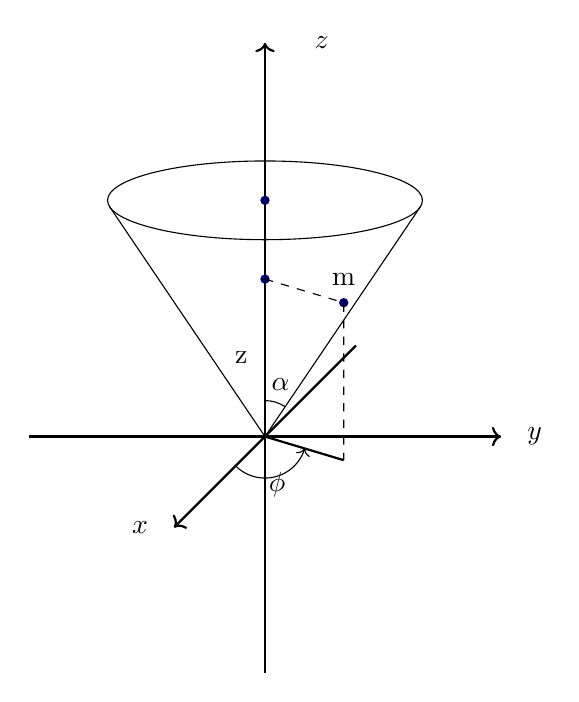
\begin{tikzpicture}
\coordinate (O) at (0,0,0);
%\tdplotsetcoord{P}{.8}{55}{60}
\draw[thick,->] (-3,0,0) -- (3,0,0) node[right =0.2]{$y$};
\draw[thick,->] (0,-3,0) -- (0,5,0) node[right= 0.5]{$z$};
\draw[thick,->] (0,0,-3) -- (0,0,3) node[left=0.2]{$x$};


\def\rx{2}    % horizontal radius of the ellipse
\def\ry{0.5}  % vertical radius of the ellipse
\def\z{3}     % distance from center of ellipse to origin
\def\p{3}  % the point on the surface
\def\pp{1.7} % the point z 
\def\ppp{1}    % the point m 
\def\ang{90}
\coordinate (p1) at (0,\p,0); 
\coordinate (p2) at (0,2,0); 
\coordinate (p3) at (\ppp,\pp,0); 
\coordinate (o) at (0,0,0);
\coordinate (y) at (0,0,1);
\coordinate (mm) at (1,-0.3,0);
\coordinate (mmm) at (1,1.5,0);
\node[fill=blue!40!black,circle,inner sep=1.2]  at (p1) {};
\node[fill=blue!40!black,circle,inner sep=1.2] (p2') at (p2) {};
\node[fill=blue!40!black,circle,inner sep=1.2] (p3') at (p3) {};
\node[above =0.1] at (p3') {m};
\node[left =0.1] at (0,1,0) {z};
\path[name path=ellipse] (0,\z) ellipse ({\rx} and {\ry});
\path[name path=horizontal] (-\rx,\z-\ry*\ry/\z) -- (\rx,\z-\ry*\ry/\z);
\path [name intersections={of = ellipse and horizontal}];
\draw[dashed] (0,2,0) -- (1,1.7,0) -- (1,-0.3,0);
\draw (intersection-1) -- (0,0) -- (intersection-2);
\draw (0,\z) ellipse ({\rx} and {\ry}); 
\draw[-,thick] (0,0,0)  -- (1,-0.3,0);
\draw pic[->,"$\phi$",draw=black,angle radius=15,angle eccentricity=1.2] {angle=y--o--mm};
%\draw pic[-,"$\alpha$",draw=black,angle radius=10,angle eccentricity=1.2] {angle=p2--o--mmm};
\draw pic[-,"$\alpha$",draw=black,angle radius=13,angle eccentricity=1.5] {angle=mmm--o--p2};
\end{tikzpicture} 




\end{document}